As outlined in the problem statement, over the years, Google has been building
its own distinctively designed data centers, deploying numerous machines around
the world. Within these facilities, arrays of servers operate continuously,
fueling essential services that a multitude of people rely on daily.
Nevertheless, the process of designing data centers is a complex optimization
challenge with multiple factors to consider.~While the primary objective is to
optimize the utilization of computing capacity offered to users, it is equally
imperative to ensure the uninterrupted provision of computing power, even in
scenarios where hardware failures are inevitable.~Drawing inspiration from
these engineering challenges, this problem presents a Google Data Center design
scenario that mirrors real-world complexities, as we describe next.

The data center, as outlined in the problem statement, is modelled as collection
of distinct~\textit{rows}. Each row consists of a specific number of
\textquote{slots}, designated for the placement of servers.~Notably, this number
of slots remains consistent across all rows within the data
center.~Additionally, certain slots within the data center may be unusable due
to other installations that impose restrictions on the utilization of those
specific spaces. However, because rows share resources, such as electrical
power, a hardware failure in one row can render the entire row of servers
inoperable.

In~\Cref{fig:data-center-layout}, an illustration depicts a layout featuring two
rows, each consisting of a total of seven slots. Note that some of these slots
are marked as unavailable, as indicated by the cross symbol.

\begin{figure}[h]
  \centering
  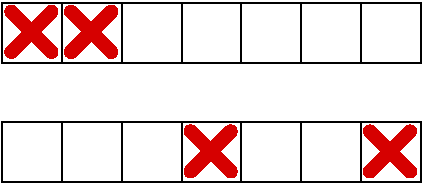
\includegraphics[width=0.6\textwidth,keepaspectratio]{../assets/dc/dc-rows-no-labels.pdf}
  \caption{Example Data Center Layout}
  \label{fig:data-center-layout}
\end{figure}

The~\emph{servers} are defined by a tuple that includes two attributes: the
\textit{size} of the server, which is measured in terms of the number of
consecutive slots occupied by the machine, and the computing~\textit{capacity}
of the server, represented as an integer value that indicates the machine's CPU
resources. Henceforth, we shall denote as $\mathcal{M}$ the total number of
servers, and use $\ell_{m}$ and $c_{m}$ to represent the~\emph{size}
and computing ~\emph{capacity} of each server ($m = 1, \ldots, \mathcal{M}$), respectively.

For illustration purposes,~\Cref{tab:dc-example-properties} presents potential
values for the aforementioned parameters, showcasing examples of four distinct
servers.

\begin{table}[ht]
  \centering
  \begin{tabular}{ccc}
  \toprule Server & Size &
  Capacity                    \\ \midrule
  1               & 3    & 2  \\
  2               & 2    & 5  \\
  3               & 3    & 10 \\
  4               & 2    & 3  \\
  \bottomrule
\end{tabular}
  \caption{Server Properties}
  \label{tab:dc-example-properties}
\end{table}

When servers are positioned within the data center rows, they are
logically associated with resource~\textit{pools}, to which they can contribute
their individual computing capacities.~The capacity of a pool is defined as the
collective sum of the capacities of all the servers allocated to it.

For clarification,~\Cref{fig:data-center-layout-with-servers} offers a potential
assignment of servers based on the data center layout depicted in
~\Cref{fig:data-center-layout}, and the server attributes provided
in~\Cref{tab:dc-example-properties}.~In this particular instance, servers are
distributed across two separate resource pools, resulting in a total capacity of
15 and 5 for pools numbered 1 and 2, respectively.

\begin{figure}[h]
  \centering
  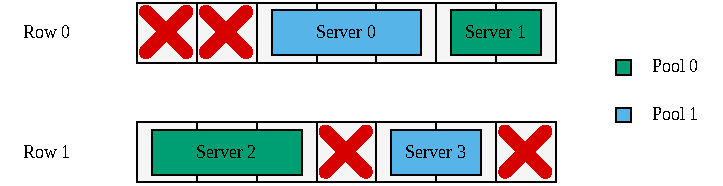
\includegraphics[width=0.9\textwidth,keepaspectratio]{../assets/dc/dc-example.pdf}
  \caption{Example Server Assignment}
  \label{fig:data-center-layout-with-servers}
\end{figure}

By examining~\Cref{fig:data-center-layout-with-servers}, it becomes evident that
the number of available slots for a row does not solely determine the constraint
for placing servers. In reality, the presence of unavailable slots can further
limit this placement, even if the total number of slots in that row would
otherwise allow it. Consequently only the set of contiguous slots within each
row, which we refer to as~\emph{segments}, can be considered.

Another important aspect is that ensuring the reliability of a specific
resource pool implies the distribution of servers across various rows.~This
strategy ensures that in the event of a row failure, the pool can still operate
with diminished capacity, drawing upon the servers located in the unaffected
rows.~In the context of the problem, this represents the concept of
a~\textit{guaranteed capacity} for a pool.

Let,~$\mathcal{P}$ be the number of resource pools,~$\mathcal{R}$ the number of
rows,~$\mathcal{I}$ the number of segments, $\mathcal{L}$ the set containing the
size (in slots) of each segment~($i = 1, \ldots, \mathcal{I}$), and
$\mathcal{I}^{r}$ the set containing the indices of all segments for a given
row~($r = 1, \ldots, \mathcal{R}$). The guaranteed capacity,~$gc_{p}$, of a
pool~($p = 1, \ldots, \mathcal{P}$) is a measure of the remaining computing
capacity available in the event that at most one arbitrary row of the data
center becomes inoperable.~Formally, this can be described as shown
in~\Cref{eq:guaranteed-capacity} where,~$x_{m,p,i}$, is a binary variable
indicating whether the server,~$m$, is assigned (1) or not (0) to pool,~$p$, and
segment~$i$.

\begin{equation}
  \label{eq:guaranteed-capacity}
  \begin{aligned}
    gc_p(x)     = & \sum_{m=1}^\mathcal{M} \sum_{r=1}^\mathcal{R} \sum_{i \in \mathcal{I}^{r}} c_m \cdot x_{m,p,i} - \max_{r=1}^\mathcal{R} \sum_{m=1}^\mathcal{M} \sum_{i \in \mathcal{I}^r} c_m \cdot x_{m,p,i} \\
  \end{aligned}
\end{equation}

In simple terms, the leftmost part of~\Cref{eq:guaranteed-capacity} represents
the capacity assigned to pool $p$, and the rightmost part indicates the capacity
that pool $p$ loses if the row with the highest capacity contribution to that
pool becomes unavailable.

The objective of this problem can thus be succinctly described as: given a
layout description of a data center, determine the optimal arrangement of
servers to data center rows and resource pools, such that, the minimum
guaranteed capacity across all pools is maximized.~Mathematically, this can be
expressed as shown in~\Cref{eq:objective}.

\begin{equation}
  \label{eq:objective}
  \begin{aligned}
    \max\ f(x)   & = \min_{p=1}^\mathcal{P}{gc_{p}(x)}                                                                                              \\
    \text{s.t. } & \sum_{p=1}^{\mathcal{P}} \sum_{r=1}^{\mathcal{R}} \sum_{i \in I^{r}} x_{m,p,i} \le 1         & \forall\ m=1,\ldots,\mathcal{M}   \\
                 & \sum_{m=1}^{\mathcal{M}} \sum_{p=1}^{\mathcal{P}} \ell_m \cdot x_{m,p,i} \le \mathcal{L}_{i} & \forall\  i=1,\ldots, \mathcal{I} \\
                 & x \in {\{0,1\}}^{\mathcal{M} \times \mathcal{P} \times \mathcal{R}}                                                              \\
  \end{aligned}
\end{equation}

Note that, the constraints encapsulate the fundamental conditions that a server,
once assigned to a specific row and segment, cannot be reassigned elsewhere, and
that the sum of the sizes of of servers allocated to a particular segment must
not exceed its predefined size.

To demonstrate the evaluation of the objective, consider the capacities assigned
to each resource pool per row as showcased in~\Cref{tab:dc-example-properties}.
The resulting objective value for this server placement is determined as
$\min(5, 2) = 2$.

\begin{table}[ht]
  \centering
  \begin{tabular}{@{\extracolsep{4pt}}cccccc@{\extracolsep{4pt}}}
  \toprule
  Pool & Row 1 & Row 2 & Guaranteed Capacity & \textbf{$f(x)$}              \\ \midrule
  1    & 5     & 10    & 5                   &                              \\
  2    & 2     & 3     & 2                   & \multirow{-2}{*}{\textbf{2}} \\
  \bottomrule
\end{tabular}
  \caption{Guaranteed Capacity \& Score}
  \label{tab:dc-gc-example}
\end{table}

Lastly, it is important to note that several instance-specific constraints
are applied to various parameters that define the data center design within
the context of this problem. These constraints are outlined as follows:

\begin{description}
  \item[\textbf{$\mathcal{R}$.}] The number of rows in the data center~($ 1 \leq \mathcal{R} \leq 1000$)
  \item[\textbf{$\mathcal{K}$.}] The number of slots in each row of the data center~($ 1 \leq \mathcal{K} \leq 1000$)
  \item[\textbf{$\mathcal{U}$.}] The number of unavailable slots~($ 0 \leq \mathcal{U} \leq \mathcal{R} \times \mathcal{K}$)
  \item[\textbf{$\mathcal{P}$.}] The number of resource pools~($ 1 \leq \mathcal{P} \leq 1000$)
  \item[\textbf{$\mathcal{M}$.}] The number of servers to be allocated~($ 1 \leq \mathcal{M} \leq \mathcal{R} \times \mathcal{K}$)
\end{description}